% !TeX program = xelatex
\documentclass[UTF8,a4paper,zihao=-4]{ctexart}

\usepackage{geometry}
\usepackage{setspace}
\usepackage{fancyhdr}
\usepackage{graphicx}
\usepackage{booktabs}
\usepackage{array}
\usepackage{longtable}
\usepackage{amsmath,amssymb}
\usepackage{float}
\usepackage{caption}
\usepackage{hyperref}
\usepackage[backend=biber,style=gb7714-2015,gbnamefmt=lowercase]{biblatex}

\geometry{left=2.5cm,right=2.5cm,top=2.5cm,bottom=2.5cm}
\setstretch{1.0}
\pagestyle{fancy}
\fancyhf{}
\fancyfoot[C]{\thepage}
\renewcommand{\headrulewidth}{0pt}
\raggedbottom
\addbibresource{references.bib}
\graphicspath{{figures/}{../figures/}}

\ctexset{
  section = {
    format = \centering\zihao{4}\heiti,
    name = {},
    number = \chinese{section}、,
    aftername = {}
  },
  subsection = {
    format = \zihao{-4}\heiti\bfseries,
    name = {},
    number = \arabic{section}.\arabic{subsection},
    aftername = { },
    beforeskip = 0.8ex plus 0.2ex minus 0.2ex,
    afterskip = 0.5ex plus 0.1ex
  },
  subsubsection = {
    format = \zihao{-4}\heiti\bfseries,
    name = {},
    number = （\arabic{subsubsection}）,
    aftername = {},
    beforeskip = 0.6ex plus 0.2ex minus 0.2ex,
    afterskip = 0.4ex plus 0.1ex
  }
}

\captionsetup{font=small,labelsep=quad}
\setCJKfamilyfont{zhhei}[AutoFakeBold=2.5]{SimHei}
\newcommand{\teamid}{请填写18位参赛队号}
\newcommand{\papertitle}{智慧烧结低碳排放的过程调控数学模型}
\newcommand{\CO}{CO}
\newcommand{\kpa}{KPa}

\begin{document}

\setcounter{page}{1}
\begin{center}
\vspace{1.0em}
{\zihao{3}\heiti \papertitle}

\vspace{2.0em}
{\zihao{3}\heiti 摘\quad 要}
\end{center}

烧结过程的烟气排放受料层状态、抽风负压、温度场和大烟道工况共同影响，变量多、耦合强，并且具有明显的时间滞后。本文围绕外排 \CO 浓度降低这一目标，先对风箱温度和 \CO 浓度建立预测模型，再在预测模型基础上给出风箱负压的调控范围和推荐方案。

针对问题一，在原始数据清洗和南北侧温度合并的基础上，分别构造局部负压滞后、相邻风箱负压滞后、全局负压滞后以及温度状态-相邻负压滞后四类特征。比较结果表明，仅使用负压变量难以解释风箱温度的热惯性；加入自身温度历史状态后，模型精度明显提高。最终采用温度状态-相邻负压滞后模型，各风箱平均 MAE 为 5.024，平均 RMSE 为 8.362，平均 $R^2$ 为 0.807。

针对问题二，将 \CO 浓度预测分为在线监测模型和调控优化模型。在线监测模型允许使用历史 \CO 项，适合报警与趋势预报；调控优化模型不使用历史 \CO 项，以避免控制变量的作用被上一时刻排放浓度掩盖。在线监测中，含 1、5、10 阶 \CO 滞后项的随机森林模型效果最好，测试集 RMSE 为 200.483，$R^2$ 为 0.838；调控优化中，剔除异常 \CO 点后的梯度提升树模型表现相对稳定，RMSE 为 475.622。

针对问题三，以调控优化模型为 \CO 响应函数，在历史 5\%-95\% 分位范围和参考工况邻域约束下，建立以预测 \CO 浓度最小为目标的风箱负压优化模型，并采用差分进化算法求解。对中位 \CO、高 \CO 和末端三类典型工况进行检验，高 \CO 工况下预测 \CO 浓度由 5091.006 mg/m$^3$ 降至 4454.131 mg/m$^3$，降幅约 12.51\%。稳健性分析表明，异常 \CO 段对模型有明显干扰；历史 \CO 项显著提高在线监测精度，但不宜直接进入调控决策模型。

\vspace{1em}
\noindent\heiti 关键词：\songti 烧结过程；风箱负压；\CO 浓度预测；时滞建模；随机森林；差分进化

\newpage

\section{问题重述}

\subsection{研究背景}

随着钢铁行业绿色低碳转型进程不断加快，传统高能耗、高排放生产方式面临越来越严格的环保约束。在“双碳”目标和超低排放改造要求的背景下，钢铁企业不仅需要保障烧结矿质量和生产稳定性，还需要进一步降低烧结烟气污染物排放水平。烧结工序作为钢铁生产流程中的重要环节，其烟气中 CO 原始排放浓度通常较高，是钢铁行业 CO 排放的重要来源之一。已有研究表明，燃料结构和操作参数会显著影响烧结过程燃烧状态和污染物排放水平\cite{ni2019fuel,wang2022coemission,zhou2020biomass}。河北省作为我国重要钢铁生产基地，已对烧结烟气 CO 排放提出明确限值要求，唐山、邯郸等钢铁产业集群城市的烧结烟气 CO 排放浓度需控制在规定标准以内。因此，如何在保证烧结过程稳定运行的同时降低 CO 排放浓度，是当前钢铁企业智能化、绿色化改造中亟需解决的问题。

烧结过程是一个多变量耦合、非线性强、动态时滞明显的复杂工业过程。烧结机机速、各风箱负压、风箱温度、大烟道负压和温度等参数共同影响料层燃烧状态、气流分布和烟气成分变化。烧结床内部温度和氧势随时间、空间不断变化，相关测量研究也说明了烧结过程条件具有明显的动态非均匀性\cite{nicol2019measurement}。其中，风箱系统连接料层燃烧反应与主抽风系统，不同风箱负压的变化会直接影响局部区域供氧条件和燃料燃烧充分程度。当风箱负压分布不合理时，料层内部容易出现局部缺氧，使燃料不完全燃烧并产生较高浓度 CO；而合理调节风箱负压能够改善料层透气性，促进 CO 进一步氧化，从而降低大烟道外排 CO 浓度。

随着钢铁企业数字化和智能化水平不断提高，烧结生产过程中可采集的运行数据逐渐丰富，包括原料状态、设备运行参数、风箱负压与温度、大烟道状态以及烟气排放浓度等时间序列数据。这些数据能够反映烧结过程的动态变化规律，为建立数据驱动的预测模型和优化调控模型提供了基础。近年来，深度学习和数据驱动方法已逐步用于烧结过程质量预测、状态识别和过程优化\cite{gong2024deeplearning}。由于烧结物料沿烧结机方向连续运动，各风箱所处空间位置不同，其负压和温度对 CO 浓度的影响具有明显的传递性和滞后性。因此，结合烧结过程数据分析风箱负压、风箱温度与 CO 排放之间的关系，对于实现烧结烟气 CO 浓度预测和风箱负压协同调控具有重要意义。

\begin{figure}[H]
  \centering
  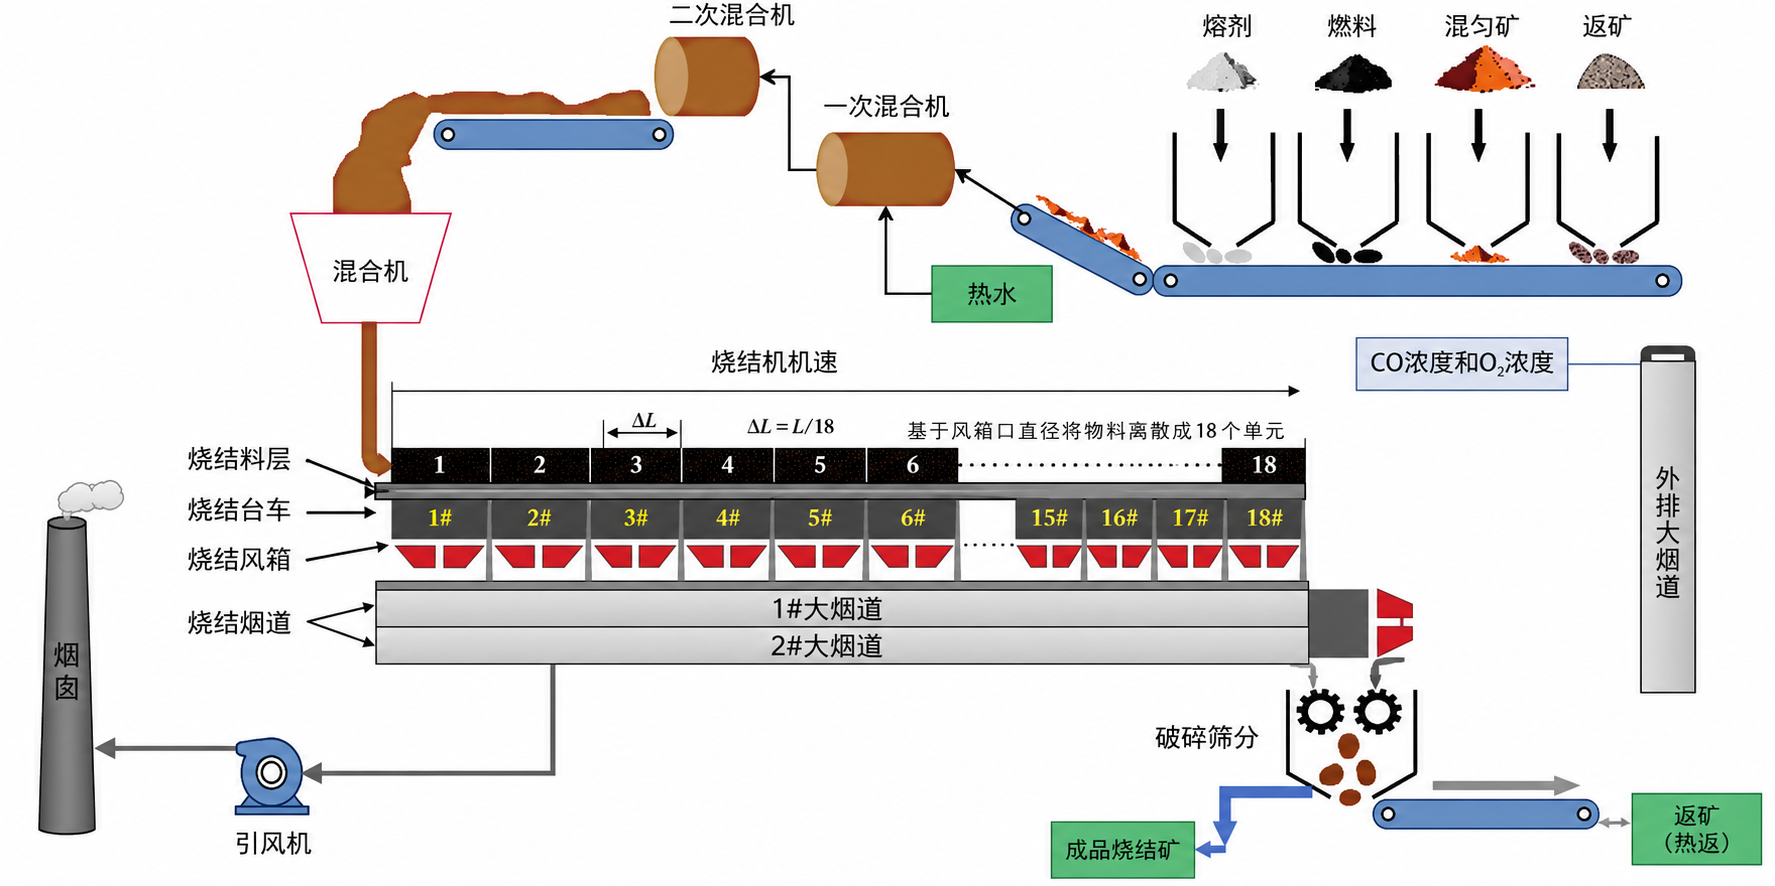
\includegraphics[width=0.75\textwidth]{背景图.png}
  \caption{烧结工艺流程及风箱-大烟道结构示意图}
  \label{fig:sintering-process}
\end{figure}

\subsection{提出问题}

为了实现烧结过程 \CO 排放浓度的预测和调控，本文依次解决以下问题。

（1）分析各风箱负压与对应风箱温度之间的关系并预测

根据给定的烧结过程时间序列数据，首先对各风箱南北两侧温度进行合并处理，得到能够代表对应风箱热状态的温度变量。在此基础上，分析不同风箱负压变化对相应风箱温度的影响规律，考虑烧结过程中的动态滞后特征，建立由风箱负压预测对应风箱温度的数学模型，并对模型的预测精度进行评价。

（2）分析烧结运行参数对大烟道外排 \CO 浓度的影响

根据各风箱负压、风箱温度以及 1\#、2\# 大烟道负压和温度等运行参数，研究其与烧结大烟道外排 \CO 浓度之间的关系。由于各风箱在烧结机上的分布位置不同，且与外排烟气检测位置之间存在距离差异，需要考虑参数影响的时滞性，通过数据配准和特征构造建立 \CO 浓度实时预测模型，用于描述烧结过程运行状态与烟气排放浓度之间的映射关系。

（3）制定降低 \CO 浓度的风箱负压调控方案

在前述 \CO 浓度预测模型的基础上，根据给定数据确定各风箱负压的合理调节范围。进一步以降低烧结大烟道外排 \CO 浓度为目标，以各风箱负压为主要调控变量，构建负压优化调控模型，求解使 \CO 排放浓度尽可能降低的风箱负压组合，并给出相应的调控决策方案。

\section{问题分析}

\subsection{问题一分析}

问题一要求探索各风箱负压与对应风箱温度之间的关系，并建立由风箱负压预测风箱温度的模型。题中给出的风箱温度包含南侧温度和北侧温度，二者均反映同一风箱附近料层燃烧和烟气热状态。为了使温度变量与风箱负压形成较清晰的对应关系，首先需要对南北两侧温度进行合并，得到每个风箱的代表温度。这样既能减少局部测点波动对模型的干扰，也能降低模型输入输出之间的复杂度。

风箱负压反映局部抽风强度，风箱温度反映对应位置的热状态。负压变化会影响料层透气性、供氧条件和燃烧带推进过程，温度变化则具有一定的热惯性和滞后性。因此，本题可以按照时间序列建模思路展开：先整理各风箱负压和合并后的风箱温度数据，再围绕当前风箱负压、历史负压、相邻风箱负压以及温度历史状态构造候选特征，最后以对应风箱温度作为预测目标建立模型，并通过误差指标评价模型对风箱热状态变化的刻画效果。

\subsection{问题二分析}

问题二要求分析各风箱负压、风箱温度以及 1\#、2\# 大烟道负压和温度对烧结大烟道外排 \CO 浓度的影响，并建立 \CO 浓度实时预测模型。外排 \CO 浓度是烧结料层燃烧、风箱抽风和大烟道汇集共同作用后的结果，烧结 CO 排放会随燃料条件、料层状态和操作参数改变而变化\cite{wang2022coemission}。因此需要分别考察风箱负压所代表的抽风状态、风箱温度所代表的热状态以及大烟道负压和温度所代表的烟气汇集状态，并将这些变量组合起来分析其对 \CO 浓度变化的共同影响。

由于 18 个风箱沿烧结机长度方向依次分布，各风箱距离外排烟气检测位置不同，且物料移动、燃烧带推进和烟气汇集均需要一定时间，所以不同位置风箱参数对最终 \CO 浓度的影响具有先后差异。靠前风箱的负压和温度变化通常需要经过较长传递过程才反映到外排 \CO 浓度中，靠后风箱的影响则相对更快。因此，需要按照时间序列数据配准的思路，为不同风箱负压、风箱温度和大烟道参数构造相应的滞后特征，使运行参数与外排 \CO 浓度在时间上形成更合理的对应关系。

在完成变量整理和时滞配准后，可将风箱负压、合并后的风箱温度、1\# 和 2\# 大烟道负压与温度作为主要输入变量，建立 \CO 浓度预测模型，并通过模型误差评价其实时预测效果。同时，\CO 浓度自身具有连续变化特征，历史 \CO 浓度可用于刻画短时排放惯性，适合与上述工艺变量共同用于实时监测；而在后续负压调控中，则应突出风箱负压等可调变量对 \CO 浓度的作用关系。通过两类变量搭配和模型比较，最终分析各运行参数对 \CO 浓度的影响规律，并得到可服务于实时预测和调控优化的 \CO 浓度模型。

\subsection{问题三分析}

问题三要求根据给定数据确定各风箱负压的调节范围，并借助问题二得到的 \CO 浓度预测模型，求解使 \CO 排放浓度尽可能低的风箱负压调控方案。与前两问不同，问题三不仅要求模型能够预测，还要求预测模型能够用于决策。因此，首先明确烧结机机速、风箱温度和大烟道状态在短时间内通常难以直接作为决策量，而风箱负压是可在线监测和调节的关键操作变量，故将 18 个风箱负压作为主要决策变量。

风箱负压的调节不能脱离实际生产范围。若优化时允许负压任意变化，可能得到虽然数学上使 \CO 浓度降低、但现场不可执行的方案。因此，需要根据历史运行数据统计各风箱负压的分布区间，并结合异常值处理结果确定合理上下限，同时限制搜索范围和相邻风箱跳变，使优化结果保持在已有生产经验和设备能力允许的范围内。

在确定调节范围后，将问题二建立的调控型 \CO 预测模型作为目标函数中的响应关系，以预测 \CO 浓度最小为目标建立优化模型。求解时固定当前工况下的机速、温度和大烟道参数，仅改变风箱负压组合，通过搜索满足约束条件的负压方案得到推荐调控结果。最后比较优化前后的预测 \CO 浓度，并分析各风箱负压变化方向和幅度，从而判断该调控方案是否具有降低排放浓度的实际意义。

\section{名词解释}

\begin{enumerate}
  \item 烧结过程：将含铁原料、熔剂和燃料按比例混合后，经点火和抽风燃烧形成烧结矿的过程。该过程沿烧结机长度方向逐步推进，具有明显的空间分段特征。
  \item 风箱负压：烧结机各风箱在抽风作用下形成的负压值，反映局部抽风强度。负压越低，通常表示抽风作用越强，但过强或过弱均可能影响燃烧充分性和料层透气性。
  \item 风箱温度：风箱南北侧温度的平均值，用于描述该风箱对应位置烟气和料层热状态。温度变化通常具有延迟性，不完全由当前负压决定。
  \item 大烟道外排 \CO 浓度：烧结烟气经大烟道汇集后的 \CO 排放浓度，是本文主要预测和优化目标。
  \item 在线监测模型：以提高短时预测精度为目的的模型，可使用历史 \CO 浓度作为输入，主要用于趋势预报和异常预警。
  \item 调控优化模型：以分析控制变量作用为目的的模型，不使用历史 \CO 浓度，主要用于风箱负压推荐。
  \item 滞后特征：将某变量前若干个采样时刻的值作为当前时刻输入，用于描述烧结过程中的传热、气流和烟气响应延迟。
\end{enumerate}

\section{模型的假设}

为便于建模和计算，作如下假设：

\begin{enumerate}
  \item 原始数据按时间顺序排列，相邻样本采样间隔为 2 s；
  \item 同一风箱南北侧温度的平均值可代表该风箱主要热状态；
  \item 建模时间段内烧结机设备运行方式未发生根本改变，历史分位范围可作为负压可调范围的参考；
  \item \CO 浓度极端低值和极端高值可能对应非稳态或检测异常，主模型采用剔除异常后的数据，并保留对比分析；
  \item 在短时负压优化中，机速、温度和大烟道状态视为给定工况，优化变量只取 18 个风箱负压。
\end{enumerate}

\section{符号说明}

\begin{longtable}{c p{9cm} c}
\caption{主要符号说明}\\
\toprule
符号 & 含义 & 单位 \\
\midrule
\endfirsthead
\caption[]{主要符号说明（续）}\\
\toprule
符号 & 含义 & 单位 \\
\midrule
\endhead
\bottomrule
\endfoot
$t$ & 时间序号，相邻时刻间隔 2 s & -- \\
$P_i(t)$ & 第 $i$ 个风箱在 $t$ 时刻的负压 & \kpa \\
$T_i(t)$ & 第 $i$ 个风箱南北侧平均温度 & $^\circ$C \\
$C(t)$ & 大烟道外排 \CO 浓度 & mg/m$^3$ \\
$v(t)$ & 烧结机机速设定值 & m/min \\
$D(t)$ & 大烟道负压和温度等状态变量 & -- \\
$\tau$ & 滞后步数 & 2 s/步 \\
$\hat C(t)$ & 模型预测的 \CO 浓度 & mg/m$^3$ \\
$\mathbf P$ & 18 个风箱负压组成的向量 & \kpa \\
\end{longtable}

\section{模型的建立与求解}

\subsection{模型数据预处理}

附件 1 给出了烧结过程中的连续时间序列数据，主要包括烧结机机速、各风箱负压、各风箱南北两侧温度、大烟道负压、大烟道温度以及大烟道外排 \CO 浓度等信息。后续将根据已知数据和需求建立模型并实现预测计算。

根据三个问题的不同目标对原始数据进行准备：

\textbf{问题一}关注风箱负压与对应风箱温度之间的关系，因此需要先将同一风箱南北两侧温度合并为代表温度，并整理各风箱负压与温度之间的对应关系。

\textbf{问题二}关注多类运行参数对外排 \CO 浓度的影响，因此需要对风箱负压、风箱温度、大烟道参数和 \CO 浓度进行变量归类，并结合风箱位置差异构造时间滞后配准变量。

\textbf{问题三}需要在 \CO 预测模型基础上进行负压调控，因此还需根据历史数据确定风箱负压的可调范围，并对可能影响模型稳定性的异常候选点进行标记。

\subsubsection{变量归类}

根据烧结工艺含义和三个问题的建模需要，将附件中的变量分为控制变量、状态变量、目标变量和派生变量四类。控制变量主要反映可调运行条件，状态变量反映当前热工和烟气状态，目标变量为需要预测或优化的结果，派生变量则由原始数据加工得到，用于补充空间位置和时间滞后信息。

\begin{longtable}{p{2.5cm} p{5.2cm} p{6.0cm}}
\caption{建模前变量归类}\\
\toprule
变量类别 & 原始字段 & 建模前处理 \\
\midrule
\endfirsthead
\caption[]{建模前变量归类（续）}\\
\toprule
变量类别 & 原始字段 & 建模前处理 \\
\midrule
\endhead
\bottomrule
\endfoot
时间变量 & 序列号 & 按 2 s 采样间隔转化为时间序号 $t$，保留样本先后顺序 \\
控制变量 & 烧结机机速、18 个风箱负压、1\# 和 2\# 大烟道负压 & 统一记号，风箱负压作为问题一、二输入变量和问题三主要调控变量 \\
状态变量 & 18 个风箱南北两侧温度、1\# 和 2\# 大烟道温度 & 将同一风箱南北侧温度合并为风箱代表温度 \\
目标变量 & 烧结大烟道外排 \CO 浓度 & 作为问题二预测目标和问题三优化目标的响应量 \\
派生变量 & 风箱位置、滞后阶数、分段统计量 & 根据风箱序号、采样间隔和机速构造空间-时间相关特征 \\
\end{longtable}

其中，问题一主要使用 18 个风箱负压和 18 个风箱代表温度；问题二在问题一变量的基础上加入大烟道负压、大烟道温度和外排 \CO 浓度；问题三则以风箱负压为决策变量，以问题二建立的 \CO 浓度模型作为响应关系。因此，风箱温度合并、风箱位置整理和滞后特征构造是三问共同需要的准备内容。

\subsubsection{温度合并}

附件中每个风箱均给出南侧温度和北侧温度。由于两侧温度对应同一风箱位置，均反映该风箱附近料层和烟气热状态，故在建模前将其合并为一个风箱代表温度。记第 $i$ 个风箱在 $t$ 时刻的南侧温度为 $T_{i,S}(t)$，北侧温度为 $T_{i,N}(t)$，合并后的风箱温度为
\begin{equation}
T_i(t)=\frac{T_{i,S}(t)+T_{i,N}(t)}{2},\quad i=1,2,\ldots,18.
\end{equation}

经过该处理，36 个风箱温度字段转化为 18 个风箱温度变量。问题一中，$T_i(t)$ 为第 $i$ 个风箱温度预测模型的输出变量；问题二中，$T_i(t)$ 与风箱负压共同作为解释外排 \CO 浓度变化的状态变量。

\subsubsection{风箱位置与时滞配准}

烧结机沿长度方向布置 18 个风箱，各风箱与外排烟气检测位置之间存在空间距离，且物料随烧结机运动、烟气经大烟道汇集后才形成检测值。因此，在使用风箱负压和温度预测 \CO 浓度前，需要将空间位置差异转化为时间序列上的滞后关系。

设 $P_i(t)$ 表示第 $i$ 个风箱负压，$T_i(t)$ 表示第 $i$ 个风箱温度，$C(t)$ 表示外排 \CO 浓度。对于问题一，主要构造 $P_i(t-\tau)$、相邻风箱 $P_{i-1}(t-\tau)$、$P_{i+1}(t-\tau)$ 以及历史温度 $T_i(t-\tau)$ 等候选变量，用于刻画负压变化对温度响应的延迟。对于问题二，则根据风箱序号和检测位置的相对远近设置候选滞后阶数，使靠前风箱对应较长滞后，靠后风箱对应较短滞后，再与大烟道负压、温度及必要的历史 \CO 浓度共同组成预测变量。

由于采样间隔为 2 s，滞后 $\tau$ 步对应的实际时间为 $2\tau$ s。若结合烧结机机速 $v(t)$ 和风箱相对距离 $d_i$ 进行粗略换算，可将空间距离对应的时间滞后写为
\begin{equation}
\tau_i(t)=\operatorname{round}\left(\frac{60d_i}{2v(t)}\right),
\end{equation}
其中 $d_i$ 表示第 $i$ 个风箱到参考检测位置的等效距离。实际建模时，可在该思想基础上设置若干候选滞后阶数，再通过相关性和预测误差确定最终使用的滞后变量。

\subsubsection{异常候选点标记}

对原始数据进行初步检查可知，外排 \CO 浓度的均值为 3530.669 mg/m$^3$，最小值为 1.447 mg/m$^3$，最大值为 9998.554 mg/m$^3$。其中低于 1000 mg/m$^3$ 的样本有 14 个，高于 6000 mg/m$^3$ 的样本有 4 个。这类点与连续烧结过程中的常规排放水平差异较大，可能对应检测波动、短时非稳态或特殊工况。

在模型准备阶段，本文先将上述样本标记为异常候选点，不直接改变原始数据。后续建模时保留两套数据处理思路：一是使用原始数据建立模型，用于观察全部工况下的整体规律；二是对异常候选点进行剔除或单独检验，用于分析极端样本对预测模型和调控模型的影响。这样既保留了原始数据的信息，又为后续稳健性分析提供了基础。

\subsection{问题一：风箱温度预测模型}

\subsubsection{模型分析}

风箱温度的变化不是瞬时完成的。负压改变后，料层内气流分布和燃烧状态会逐步影响温度；同时相邻风箱之间沿烧结方向存在热状态传播。因此，仅用当前风箱当前负压解释当前温度，容易忽略系统的热惯性。

本文对四类特征方案进行比较：

\begin{enumerate}
  \item 局部负压滞后模型：只使用本风箱负压及其滞后；
  \item 相邻风箱空间滞后模型：加入前后相邻风箱负压；
  \item 全局风箱空间滞后模型：加入全部风箱负压；
  \item 温度状态-相邻负压滞后模型：加入本风箱历史温度和相邻风箱负压滞后。
\end{enumerate}

\subsubsection{模型建立}

对第 $i$ 个风箱建立预测函数：
\begin{equation}
\hat T_i(t)=f_i\left(T_i(t-1),T_i(t-5),T_i(t-10),P_{i-1}(t-\tau),P_i(t-\tau),P_{i+1}(t-\tau),v(t)\right),
\end{equation}
其中边界风箱只取存在的相邻项，$\tau\in\{0,5,10,20\}$。模型候选包括岭回归、随机森林和梯度提升树。岭回归用于刻画较稳定的线性状态延续，随机森林和梯度提升树用于刻画非线性响应\cite{breiman2001random,friedman2001greedy}。

评价指标采用 MAE、RMSE 和 $R^2$：
\begin{equation}
\mathrm{MAE}=\frac{1}{n}\sum_{k=1}^{n}|y_k-\hat y_k|,
\end{equation}
\begin{equation}
\mathrm{RMSE}=\sqrt{\frac{1}{n}\sum_{k=1}^{n}(y_k-\hat y_k)^2},\quad
R^2=1-\frac{\sum_{k=1}^{n}(y_k-\hat y_k)^2}{\sum_{k=1}^{n}(y_k-\bar y)^2}.
\end{equation}

具体求解步骤如下：

\begin{enumerate}
  \item 对每一个风箱分别建立回归模型，使模型能够适应不同位置风箱的温度水平和波动幅度；
  \item 对四类特征方案分别训练模型，并在同一测试集上计算 MAE、RMSE 和 $R^2$；
  \item 对每个风箱选择测试集表现最好的模型作为该风箱温度预测模型；
  \item 汇总 18 个风箱的平均指标，用于判断整体特征方案优劣。
\end{enumerate}

这种逐风箱建模的方法比把 18 个风箱温度合并为一个大模型更稳妥。原因是不同风箱处在烧结过程的不同位置，前段更接近点火和燃烧初期，中段反映燃烧带主要通过区域，后段更多体现烟气汇集和尾部状态；若强行使用同一组参数，容易掩盖各风箱的工艺差异。

\subsubsection{结果分析}

\begin{longtable}{l r r r}
\caption{问题一不同特征方案的平均预测效果}\\
\toprule
特征方案 & 平均 MAE & 平均 RMSE & 平均 $R^2$ \\
\midrule
\endfirsthead
\caption[]{问题一不同特征方案的平均预测效果（续）}\\
\toprule
特征方案 & 平均 MAE & 平均 RMSE & 平均 $R^2$ \\
\midrule
\endhead
\bottomrule
\endfoot
温度状态-相邻负压滞后 & 5.024 & 8.362 & 0.807 \\
相邻风箱负压滞后 & 13.810 & 20.096 & -0.335 \\
局部负压滞后 & 13.988 & 20.101 & -0.290 \\
全局风箱负压滞后 & 14.962 & 25.606 & -0.823 \\
\end{longtable}

从表中可以看出，温度状态-相邻负压滞后模型明显优于其他三类方案。这说明风箱温度主要具有状态延续性，负压对温度的作用需要通过当前热状态和邻近空间状态共同体现。仅增加全部风箱负压并没有改善结果，反而引入了较多冗余变量，使模型在测试集上表现变差。

各风箱中，第 3、10、11、15 号等风箱的 $R^2$ 均超过 0.90；第 1、17 号风箱相对较低，但仍明显好于只使用负压变量的方案。由此可见，该模型能够作为后续 \CO 建模中的温度状态补充。

进一步观察各风箱结果可以发现，前段 2--8 号风箱的温度预测误差普遍较小，说明这些位置的温度变化较稳定，历史温度对当前温度具有较强解释能力；12--14 号风箱误差相对较大，可能与燃烧带位置波动和烟气汇集状态变化有关。实际应用时，可对中后段风箱设置更高的监测权重，以便及时发现热状态异常。

\subsection{问题二：\CO 浓度预测模型}

\subsubsection{滞后相关分析}

对 \CO 浓度与各工艺变量进行滞后相关扫描，绝对相关系数较高的变量主要包括前中段风箱温度、部分中段风箱负压和大烟道负压。相关系数本身并不高，最大约为 0.253，说明 \CO 浓度受多变量共同影响，单个变量难以单独解释排放波动。

\begin{longtable}{l r r r}
\caption{部分变量与 \CO 浓度的滞后相关结果}\\
\toprule
变量 & 滞后步数 & 滞后秒数 & 相关系数 \\
\midrule
\endfirsthead
\caption[]{部分变量与 \CO 浓度的滞后相关结果（续）}\\
\toprule
变量 & 滞后步数 & 滞后秒数 & 相关系数 \\
\midrule
\endhead
\bottomrule
\endfoot
4\#风箱平均温度 & 14 & 28 & 0.253 \\
7\#风箱平均温度 & 10 & 20 & 0.252 \\
14\#风箱平均温度 & 0 & 0 & -0.246 \\
6\#风箱平均温度 & 3 & 6 & 0.245 \\
10\#风箱负压 & 1 & 2 & -0.230 \\
11\#风箱负压 & 1 & 2 & -0.230 \\
1\#大烟道负压 & 1 & 2 & -0.210 \\
\end{longtable}

\subsubsection{两类预测模型的区分}

若目标是在线监测，则可以使用历史 \CO 浓度，因为实际运行中上一时刻排放值是可观测的。此时模型为
\begin{equation}
\hat C(t)=g_{\mathrm{monitor}}\left(X(t),X(t-\tau),C(t-1),C(t-5),C(t-10)\right),
\end{equation}
其中 $X(t)$ 表示负压、温度、大烟道参数和机速等工艺变量。

若目标是负压优化，则不宜使用历史 \CO 浓度。否则在优化时，模型主要根据 $C(t-1)$ 判断 $C(t)$，负压变量的调节作用会被弱化。调控模型写为
\begin{equation}
\hat C(t)=g_{\mathrm{control}}\left(v(t),P_1(t),\ldots,P_{18}(t),T_1(t),\ldots,T_{18}(t),D(t)\right).
\end{equation}

两类模型的输入虽然相近，但用途不同。在线监测模型相当于“短时预报器”，只要上一时刻的 \CO 浓度可测，就应充分利用其连续性；调控优化模型相当于“工况响应器”，重点是判断在相同温度、大烟道状态和机速条件下，负压变化会如何影响预测排放。因此，本文没有简单地选取精度最高的模型用于优化，而是将高精度模型和可调控模型分开使用。

模型训练时仍采用时间顺序划分。为降低极端点影响，调控模型优先使用剔除异常 \CO 候选点后的数据；在线监测模型也在相同异常处理基础上训练，以保证两类模型的比较口径一致。

\subsubsection{模型求解与结果}

\begin{longtable}{l l r r r}
\caption{\CO 浓度预测模型对比}\\
\toprule
用途 & 模型 & MAE & RMSE & $R^2$ \\
\midrule
\endfirsthead
\caption[]{\CO 浓度预测模型对比（续）}\\
\toprule
用途 & 模型 & MAE & RMSE & $R^2$ \\
\midrule
\endhead
\bottomrule
\endfoot
实时监测 & RF，含 \CO 滞后 1/5/10 & 114.197 & 200.483 & 0.838 \\
实时监测 & Ridge，含 \CO 滞后 1/5/10 & 143.059 & 237.588 & 0.773 \\
实时监测 & GBRT，含 \CO 滞后 1/5/10 & 142.825 & 238.035 & 0.772 \\
实时监测 & Linear，含 \CO 滞后 1/5/10 & 206.835 & 413.183 & 0.312 \\
调控优化 & GBRT，无 \CO 滞后 & 368.120 & 475.622 & 0.082 \\
调控优化 & RF，无 \CO 滞后 & 375.516 & 492.667 & 0.015 \\
\end{longtable}

实时监测模型中，随机森林的表现最好，$R^2$ 达到 0.838，说明 \CO 浓度具有较强的短期自相关特征，适合用于在线预警。调控优化模型精度明显低于监测模型，这是合理现象：在不使用历史 \CO 的条件下，模型只能依靠可调负压和可观测工况解释排放波动，而题目数据中缺少燃料配比、料层厚度、混合料水分等关键变量。因此，调控模型更适合作为负压调整的辅助工具，而非单点精确预测器。本文后续优化只在同一工况邻域内比较不同负压组合的相对优劣，并通过历史分位和参考工况邻域约束降低模型外推风险。

从模型结果看，线性回归在实时监测任务中的 $R^2$ 仅为 0.312，说明 \CO 排放与工艺变量之间并非简单线性关系。随机森林和梯度提升树均能刻画非线性关系，但随机森林在加入历史 \CO 项后更稳定，说明短时排放变化中存在较强的局部相似性。相反，在调控优化任务中梯度提升树略优于随机森林，原因可能是梯度提升树对连续控制变量的单调区间和局部响应更敏感，因而更适合作为后续优化目标函数。这与烧结过程智能建模研究中强调的非线性、强耦合和数据驱动建模特点是一致的\cite{gong2024deeplearning}。

\subsection{问题三：风箱负压优化调控模型}

\subsubsection{模型分析}

负压调控需要满足两个条件。第一，调节值不能脱离历史运行范围，否则模型外推不可靠；第二，推荐方案不能造成相邻风箱之间的剧烈跳变，否则不符合实际生产中的平稳操作原则。基于此，本文以历史 5\%-95\% 分位作为主要调控范围，并围绕当前工况的邻域给出推荐负压。若当前负压已经处于历史主要分布区间之外，则先将其拉回历史 5\%-95\% 分位区间，再在该区间内搜索局部改进方案。

需要说明的是，问题三中使用的调控模型并不追求对 \CO 浓度绝对值的最高预测精度。由于该模型不使用历史 \CO 项，其 $R^2$ 低于在线监测模型，但它保留了风箱负压、温度和大烟道状态等工艺变量对 \CO 浓度的响应关系。因此，本文将该模型用于同一工况下不同负压方案的相对比较，而不是把其预测值作为现场排放浓度的精确替代。这样处理可以避免历史 \CO 项掩盖负压调节作用，使优化结果更具有调控解释性。

\subsubsection{优化模型建立}

记 18 个风箱负压向量为
\begin{equation}
\mathbf P=(P_1,P_2,\ldots,P_{18})^\top.
\end{equation}

在给定工况 $\mathbf Z$ 下，优化目标为
\begin{equation}
\min_{\mathbf P}\quad g_{\mathrm{control}}(\mathbf P,\mathbf Z)+\lambda_1\sum_{i=1}^{18}\left(\frac{P_i-P_i^0}{r_i}\right)^2+\lambda_2\sum_{i=1}^{17}(P_{i+1}-P_i)^2.
\end{equation}
其中 $P_i^0$ 为当前负压，$r_i$ 为第 $i$ 个风箱的历史调节尺度，第二项限制调节幅度，第三项限制相邻风箱负压曲线过度跳变。

式中 $\lambda_1$ 和 $\lambda_2$ 为惩罚权重。$\lambda_1$ 用于控制推荐负压偏离当前工况的幅度，防止模型为追求较低预测 \CO 而给出过大调节；$\lambda_2$ 用于控制相邻风箱之间的负压平滑性，避免出现局部风箱突变而破坏原有抽风分布。本文通过多组典型工况试算确定权重设定原则：在保证预测 \CO 浓度下降的前提下，优先选择负压变化幅度较小、相邻风箱曲线较平滑的方案。换言之，目标函数不是单纯追求数学上的最低 \CO 预测值，而是在“降排效果”和“可执行性”之间取得折中。

约束条件为
\begin{equation}
P_i^{5\%}\leq P_i\leq P_i^{95\%},\quad
\max(P_i^{5\%},\tilde P_i^0-1.5)\leq P_i\leq \min(P_i^{95\%},\tilde P_i^0+1.5),
\quad i=1,2,\ldots,18.
\end{equation}
其中 $\tilde P_i^0=\min\{\max(P_i^0,P_i^{5\%}),P_i^{95\%}\}$，表示将当前负压 $P_i^0$ 截断到历史主要运行区间后的参考值。这样处理的含义是：若当前工况本身已经偏离常规运行范围，优化模型不再围绕异常点继续微调，而是优先给出回到历史常规区间内的推荐方向。

由于 $g_{\mathrm{control}}$ 为梯度提升树模型，目标函数不可直接写出解析梯度，因此采用差分进化算法进行求解\cite{storn1997differential}。

为降低树模型局部不连续带来的偶然性，本文在优化过程中加入两类约束：一类是历史分位约束，保证搜索范围落在样本主要分布区间内；另一类是参考工况邻域约束，保证推荐方案不脱离当前生产状态及历史经验范围。若推荐值与当前值相差较大，则不建议现场一次性调整到位，而应拆分为若干小步，并以在线 \CO 监测结果作为反馈。这样可以减少模型外推风险，也更符合烧结生产中逐步调节、观察反馈的操作习惯。

算法求解流程如下：

\begin{enumerate}
  \item 给定某一典型工况，固定机速、风箱温度和大烟道状态；
  \item 以该工况当前 18 个风箱负压作为初始参考值；
  \item 根据历史 5\%-95\% 分位和参考工况邻域确定每个风箱搜索区间；
  \item 以调控模型预测 \CO 浓度、负压变化惩罚和相邻风箱平滑惩罚构造目标函数；
  \item 采用差分进化算法在约束区间内搜索，得到推荐负压向量；
  \item 将推荐负压代回调控模型，比较优化前后预测 \CO 浓度。
\end{enumerate}

本文选择中位 \CO 工况、高 \CO 工况和末端工况进行验证。中位工况用于观察模型在常规排放水平下的调节幅度，高 \CO 工况用于检验模型在需要降排时的作用，末端工况用于检查模型对时间序列后部样本的稳定性。

\subsubsection{调控范围}

\begin{longtable}{l r r r r}
\caption{部分风箱负压调控范围}\\
\toprule
变量 & 历史最小值 & 5\%分位 & 95\%分位 & 历史最大值 \\
\midrule
\endfirsthead
\caption[]{部分风箱负压调控范围（续）}\\
\toprule
变量 & 历史最小值 & 5\%分位 & 95\%分位 & 历史最大值 \\
\midrule
\endhead
\bottomrule
\endfoot
1\#风箱负压 & -14.057 & -12.057 & -10.825 & -4.689 \\
6\#风箱负压 & -16.941 & -14.874 & -13.671 & -11.984 \\
10\#风箱负压 & -16.852 & -14.814 & -13.601 & -8.480 \\
14\#风箱负压 & -16.652 & -14.602 & -10.071 & -4.086 \\
18\#风箱负压 & -14.005 & -11.528 & -5.351 & -2.580 \\
\end{longtable}

可以看到，中段风箱负压通常更低，说明该区域抽风强度较大；后段风箱的 95\% 分位变化范围较宽，实际调节时应结合现场工艺约束进一步确认。

\subsubsection{典型工况优化结果}

\begin{longtable}{l r r r r r}
\caption{典型工况优化效果}\\
\toprule
工况 & 序列 & 真实 \CO & 优化前预测 & 优化后预测 & 降低比例 \\
\midrule
\endfirsthead
\caption[]{典型工况优化效果（续）}\\
\toprule
工况 & 序列 & 真实 \CO & 优化前预测 & 优化后预测 & 降低比例 \\
\midrule
\endhead
\bottomrule
\endfoot
中位 \CO 工况 & 30 & 3505.859 & 3481.322 & 3426.724 & 1.57\% \\
高 \CO 工况 & 2310 & 5360.243 & 5091.006 & 4454.131 & 12.51\% \\
末端工况 & 2442 & 3566.985 & 3611.766 & 3478.161 & 3.70\% \\
\end{longtable}

高 \CO 工况的优化效果最明显，预测降低量为 636.875 mg/m$^3$。这说明当排放处于较高水平时，风箱负压仍具有一定可调空间；而在中位 \CO 工况下，优化幅度较小，表明该工况已接近模型认为的相对平稳状态。由于调控模型主要用于方案排序，表中“优化后预测”应理解为模型在相同工况下对推荐负压方案的相对评价，现场执行时仍需结合实时 \CO 监测模型进行闭环校核。

\begin{figure}[H]
  \centering
  
\includegraphics[width=0.95\textwidth]{pressure_strategy.png}
  \caption{典型工况推荐负压曲线}
  \label{fig:pressure}
\end{figure}

从图 \ref{fig:pressure} 可以看出，三类工况的推荐负压曲线总体保持了烧结过程原有的分区特征。高 \CO 工况下，模型主要对中后段若干风箱进行调整，而不是对全部风箱同步改变，这与烧结烟气在中后段汇集并影响外排浓度的工艺认识基本一致。

\begin{longtable}{l r l r}
\caption{高 \CO 工况下部分风箱推荐负压}\\
\toprule
风箱 & 推荐负压 & 风箱 & 推荐负压 \\
\midrule
\endfirsthead
\caption[]{高 \CO 工况下部分风箱推荐负压（续）}\\
\toprule
风箱 & 推荐负压 & 风箱 & 推荐负压 \\
\midrule
\endhead
\bottomrule
\endfoot
1\# & -11.820 & 10\# & -14.691 \\
3\# & -11.392 & 12\# & -14.292 \\
6\# & -14.542 & 14\# & -14.174 \\
8\# & -14.306 & 16\# & -13.270 \\
9\# & -14.859 & 18\# & -11.256 \\
\end{longtable}

为进一步检查推荐方案的可执行性，表 \ref{tab:pressure_delta} 列出了高 \CO 工况下若干风箱的当前负压、推荐负压和调整量。可以看到，推荐方案并非简单增强抽风，而是将部分已经偏强的负压拉回历史主要运行区间。以 16\# 风箱为例，当前负压为 -16.369 \kpa，已低于该风箱历史 5\% 分位 -14.389 \kpa，模型推荐值为 -13.270 \kpa，属于向常规区间回调；18\# 风箱则仅作小幅增强。由此可见，优化结果的主要含义不是“全线加大负压”，而是修正高 \CO 工况下不均衡的抽风分布。

\begin{longtable}{l r r r l}
\caption{高 \CO 工况下部分风箱负压调整量核查}
\label{tab:pressure_delta}\\
\toprule
风箱 & 当前负压 & 推荐负压 & 调整量 & 调整方向 \\
\midrule
\endfirsthead
\caption[]{高 \CO 工况下部分风箱负压调整量核查（续）}\\
\toprule
风箱 & 当前负压 & 推荐负压 & 调整量 & 调整方向 \\
\midrule
\endhead
\bottomrule
\endfoot
1\# & -13.781 & -11.820 & 1.961 & 减弱抽风 \\
6\# & -16.924 & -14.542 & 2.382 & 减弱抽风 \\
10\# & -16.820 & -14.691 & 2.129 & 减弱抽风 \\
14\# & -16.623 & -14.174 & 2.449 & 减弱抽风 \\
16\# & -16.369 & -13.270 & 3.099 & 减弱抽风 \\
18\# & -10.932 & -11.256 & -0.324 & 增强抽风 \\
\end{longtable}

该推荐结果并不是简单地把所有风箱负压都调到更低，而是在前段、中段和后段之间保持差异。中段 6--14 号风箱维持较强抽风，后段部分风箱则保持相对温和的负压水平。这样处理一方面保留了烧结过程原有的通风分布，另一方面避免大幅度同步调节造成生产波动。

综合典型工况结果，本文建议将优化模型作为“推荐方向生成器”使用：当在线监测模型判断 \CO 浓度存在升高趋势时，调控模型给出当前工况附近的负压调整方向；现场执行时先按较小步长调整，例如每次仅执行推荐调整量的一部分，待 1--2 个过程滞后周期后观察 \CO 监测模型和实际检测值的响应，再决定是否继续向推荐值靠近。该使用方式比一次性采用大幅调节更稳妥，也更符合工业过程控制中的安全边界要求。

\section{模型的灵敏度分析}

参考获奖论文中对关键外部条件进行敏感性分析的写法，本文从异常样本、工艺变量滞后阶数和历史 \CO 项三个角度检验模型稳定性。这三个因素分别对应数据质量、过程时滞和排放自身惯性，是影响本文结论可靠性的主要来源。

\subsection{异常处理稳健性}

\begin{longtable}{l r r r}
\caption{异常处理对调控模型的影响}\\
\toprule
方案 & MAE & RMSE & $R^2$ \\
\midrule
\endfirsthead
\caption[]{异常处理对调控模型的影响（续）}\\
\toprule
方案 & MAE & RMSE & $R^2$ \\
\midrule
\endhead
\bottomrule
\endfoot
原始数据-Ridge & 436.278 & 645.279 & -0.699 \\
原始数据-GBRT & 392.906 & 517.414 & -0.093 \\
原始数据-RF & 383.562 & 504.262 & -0.038 \\
剔除异常 \CO-GBRT & 368.120 & 475.622 & 0.082 \\
剔除异常 \CO-RF & 375.516 & 492.667 & 0.015 \\
\end{longtable}

剔除异常候选点后，梯度提升树模型的 RMSE 从 517.414 降至 475.622，$R^2$ 由负值提升到 0.082。说明极端 \CO 样本对调控模型有明显影响，主模型采用剔除异常后的结果更稳妥。

从工艺角度看，极低 \CO 浓度可能由传感器瞬时失真、工况切换或数据记录异常造成；极高 \CO 浓度则可能对应短时非稳态燃烧。若直接纳入调控模型，模型会试图用负压和温度解释这些极端点，从而扭曲正常工况下的负压响应关系。因此，本文不删除这些信息，而是将其作为异常候选段单独分析，并在稳健性比较中说明处理前后的差异。

同时也可以看到，剔除异常后的调控模型 $R^2$ 仍然不高。本文对此不作过度回避，而是将其作为模型适用边界处理：该模型不适合单独承担排放浓度的高精度预测任务，但在限定工况邻域、限定负压调节范围时，可作为比较候选负压方案的辅助响应函数。换言之，问题二中的实时监测模型负责“看得准”，问题三中的调控模型负责“调得有依据”，二者配合使用比单一模型更稳健。

\subsection{滞后项敏感性}

\begin{longtable}{l r r r}
\caption{工艺变量滞后阶数敏感性}\\
\toprule
方案 & MAE & RMSE & $R^2$ \\
\midrule
\endfirsthead
\caption[]{工艺变量滞后阶数敏感性（续）}\\
\toprule
方案 & MAE & RMSE & $R^2$ \\
\midrule
\endhead
\bottomrule
\endfoot
无滞后 & 368.120 & 475.622 & 0.082 \\
10s/20s/40s & 378.307 & 478.031 & 0.079 \\
20s/40s/80s & 370.742 & 476.918 & 0.089 \\
40s/80s/120s & 373.857 & 486.712 & 0.059 \\
\end{longtable}

不同工艺滞后阶数下模型结果较接近，说明在当前数据粒度下，单纯增加负压和温度滞后项并不能显著提升调控模型。可能原因是外排 \CO 还受到燃料、配料和料层状态等未观测变量影响。已有烧结燃烧与排放研究也表明，燃料类型、配碳量和操作制度会共同影响燃烧过程和污染物排放\cite{ni2019fuel,zhou2020biomass}。

需要注意的是，滞后项“提升有限”并不说明烧结过程没有滞后，而是说明在当前可观测变量中，负压和温度的滞后信息不足以完全解释 \CO 排放变化。后续若能加入混合料水分、焦粉配比、料层厚度等变量，滞后结构可能会表现得更加清楚。

\subsection{\CO 历史项敏感性}

\begin{longtable}{l r r r}
\caption{\CO 历史滞后项对在线监测的影响}\\
\toprule
方案 & MAE & RMSE & $R^2$ \\
\midrule
\endfirsthead
\caption[]{\CO 历史滞后项对在线监测的影响（续）}\\
\toprule
方案 & MAE & RMSE & $R^2$ \\
\midrule
\endhead
\bottomrule
\endfoot
仅工艺变量 & 375.516 & 492.667 & 0.015 \\
工艺滞后 & 384.538 & 492.414 & 0.023 \\
\CO\_lag1 & 114.807 & 201.304 & 0.837 \\
\CO\_lag1\_5 & 114.437 & 200.979 & 0.837 \\
\CO\_lag1\_5\_10 & 114.197 & 200.483 & 0.838 \\
\end{longtable}

加入历史 \CO 后，在线监测模型精度大幅提升。这一结果说明 \CO 浓度具有很强的短时连续性。但这也进一步说明，监测模型和调控模型必须分开使用：前者追求预报准确，后者追求控制变量的可解释响应。

从表中可以看到，仅加入 1 阶历史 \CO 项后，$R^2$ 即由 0.015 提升到 0.837，继续加入 5 阶和 10 阶滞后后提升很小。这说明对 2 s 采样间隔的数据而言，最近一个采样点已经包含大部分短时排放惯性。实际部署时，在线预警可使用该模型；而负压优化仍应采用不含历史 \CO 项的模型，避免出现“预测准确但无法指导调节”的情况。

\begin{figure}[H]
  \centering
  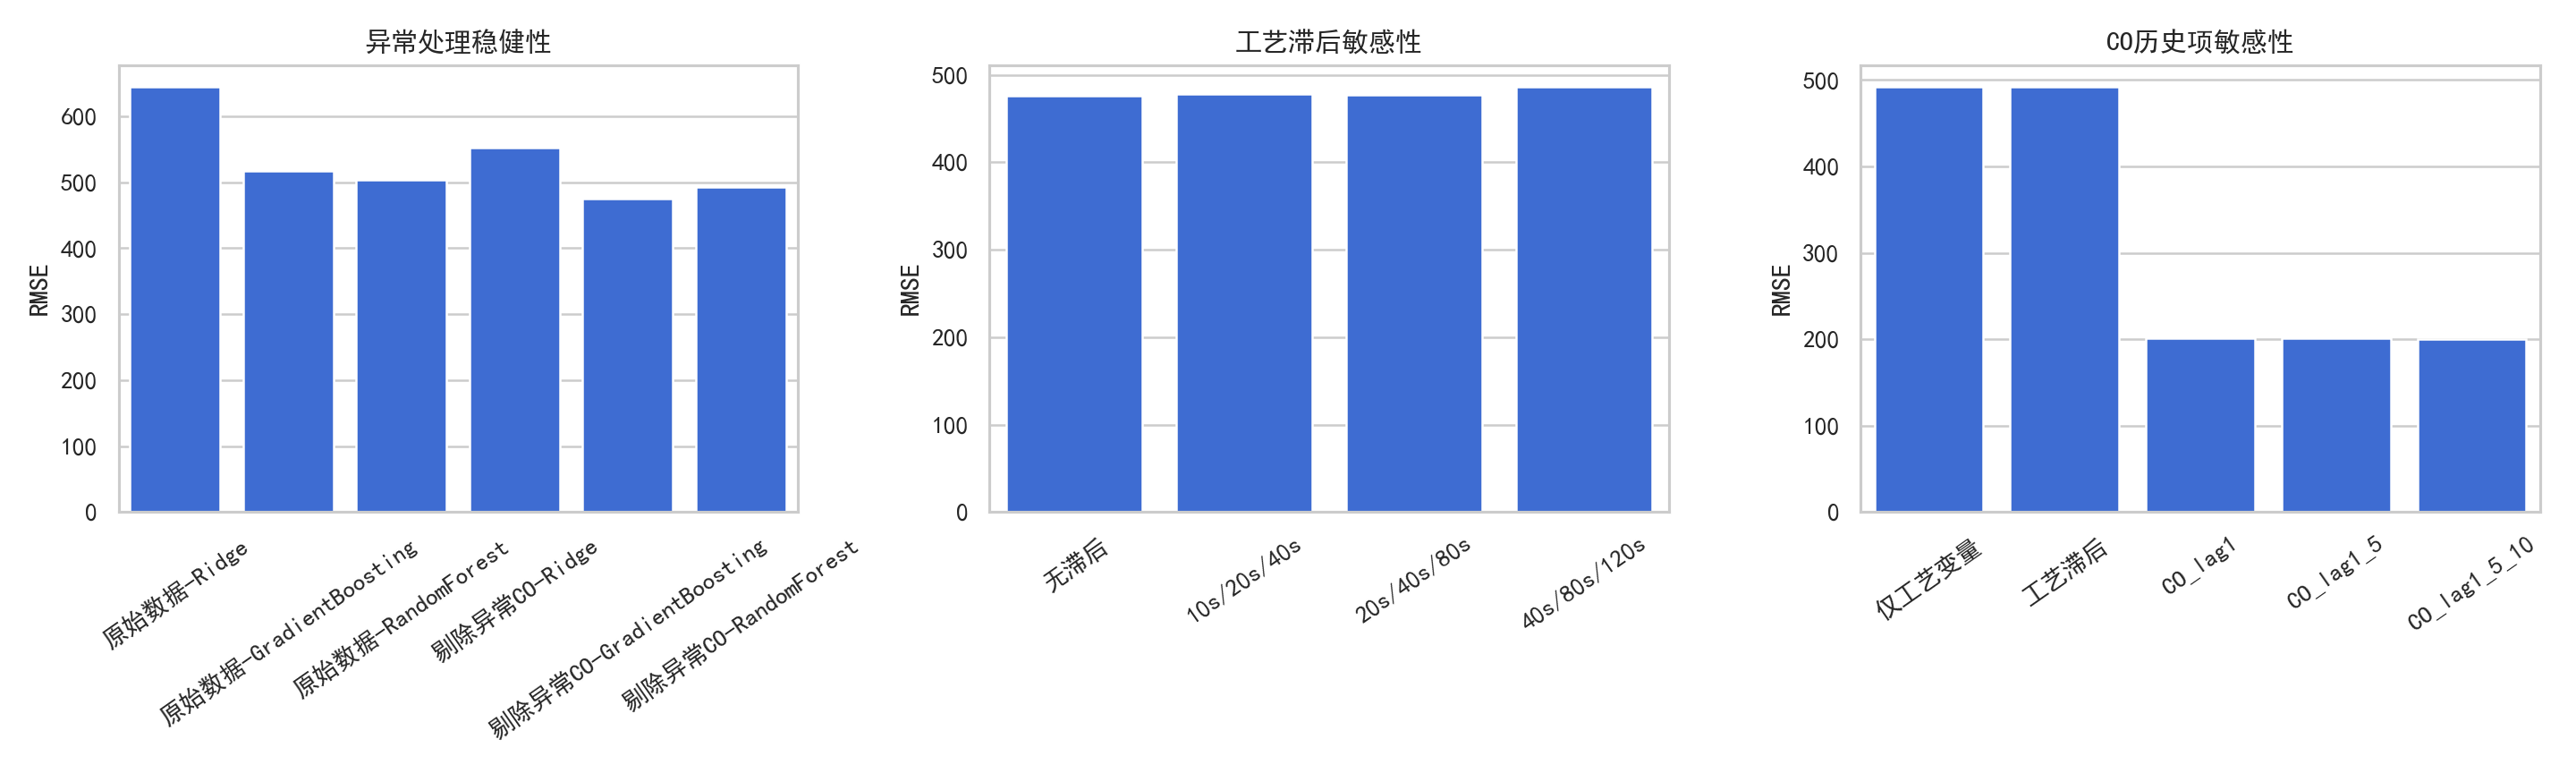
\includegraphics[width=0.95\textwidth]{robustness_rmse.png}
  \caption{稳健性分析 RMSE 对比}
  \label{fig:robustness}
\end{figure}

\section{模型的评价与推广}

\subsection{模型优点}

本文模型的主要优点有三点。第一，建模流程按烧结过程的逻辑展开，先刻画温度状态，再刻画 \CO 排放，最后进行负压优化，层次比较清楚。第二，将在线监测和调控优化区分开来，避免用高精度监测模型直接做控制决策。第三，优化约束来自历史运行分位、参考工况邻域和相邻风箱平滑要求，所得方案不脱离实际数据范围。

\subsection{模型不足}

模型也存在不足。首先，题目数据缺少燃料配比、料层厚度、混合料水分、点火温度等关键变量，调控模型对 \CO 的解释能力受到限制。其次，本文将短时优化中温度和大烟道状态视为给定工况，没有进一步模拟负压调整后温度场的反馈变化。再次，异常 \CO 样本只能根据数值范围识别，无法完全判断其来源。

\subsection{模型推广}

若用于实际生产，可在当前模型基础上增加三类信息：一是配料和燃料数据，用于提高 \CO 形成机理的解释能力；二是更长时间的连续生产数据，用于区分班次、料批和设备状态差异；三是现场控制约束，如风机能力、阀门开度和相邻风箱联动规则。这样可以将本文的静态推荐方案进一步发展为滚动优化调控模型。

\subsection{结论}

本文建立了面向智慧烧结低碳排放的过程调控模型。问题一中，温度状态-相邻负压滞后模型取得最佳效果，平均 $R^2$ 为 0.807，说明热状态历史对风箱温度预测至关重要。问题二中，含历史 \CO 项的随机森林模型适合在线监测，$R^2$ 达到 0.838；不含历史 \CO 项的梯度提升树模型用于后续负压调控，虽然精度较低，但具有更清晰的控制解释性。问题三中，在历史分位和参考工况邻域约束下，差分进化算法能够给出可执行的负压推荐方案，高 \CO 工况下预测降幅约 12.51\%。整体来看，本文方法能够为烧结过程 \CO 排放监测和负压调节提供定量依据。

\printbibliography[title={参考文献}]

\end{document}
